\documentclass[a4paper,10pt]{article}
\usepackage[utf8x]{inputenc}
\usepackage{tikz}
\usepackage{amsmath,amssymb}

\begin{document}

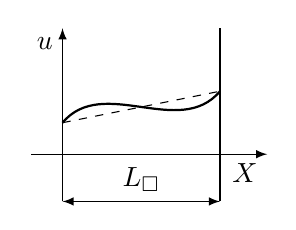
\begin{tikzpicture}[scale=2,>=latex]
 \draw[->] (-0.2,0) -- (1.3,0) node[at end,below left] {$X$};
 \draw[->] (0,-0.3) -- (0,0.8) node[at end,below left] {$u$};
 \draw[] (1,-0.3) -- (1,0.8);
 \draw[<->] (0,-0.3) -- (1,-0.3) node[midway,above] {$L_\Box$};
 \draw[dashed] (0,0.2) -- (1,0.4);

 \draw[thick] (0,0.2) to[out=50,in=-130] (1,0.4);
\end{tikzpicture}

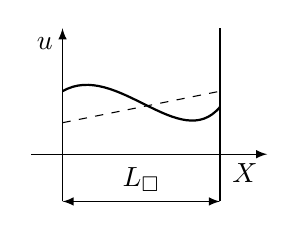
\begin{tikzpicture}[scale=2,>=latex]
 \draw[->] (-0.2,0) -- (1.3,0) node[at end,below left] {$X$};
 \draw[->] (0,-0.3) -- (0,0.8) node[at end,below left] {$u$};
 \draw[] (1,-0.3) -- (1,0.8);
 \draw[<->] (0,-0.3) -- (1,-0.3) node[midway,above] {$L_\Box$};
 \draw[dashed] (0,0.2) -- (1,0.4);

 \draw[thick] (0,0.4) to[out=30,in=-130] (1,0.3);
\end{tikzpicture}

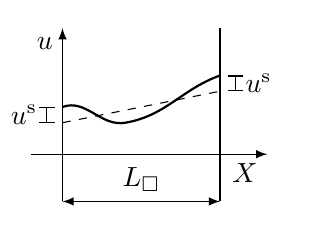
\begin{tikzpicture}[scale=2,>=latex]
 \draw[->] (-0.2,0) -- (1.3,0) node[at end,below left] {$X$};
 \draw[->] (0,-0.3) -- (0,0.8) node[at end,below left] {$u$};
 \draw[] (1,-0.3) -- (1,0.8);
 \draw[<->] (0,-0.3) -- (1,-0.3) node[midway,above] {$L_\Box$};
 \draw[dashed] (0,0.2) -- (1,0.4);

 \draw[thick] (0,0.3) to[out=20,in=-170] (0.4,0.2) to[out=10,in=-160] (1,0.5);
 \draw[|-|] (-0.1,0.2) -- (-0.1,0.3) node[midway,left] { \llap{$u^{\mathrm{s}}$} }; % llap to align figures nicely.
 \draw[|-|] (1.1,0.4) -- (1.1,0.5) node[midway,right] { $u^{\mathrm{s}}$ };
\end{tikzpicture}

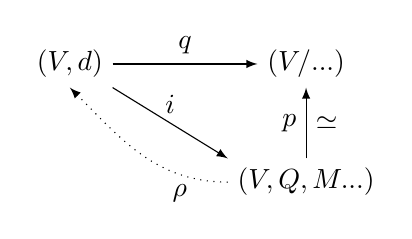
\begin{tikzpicture}[>=latex]
\node (Vd) at (0,0) {$(V,d)$}; 
\node (VVd) at (3,0) {$(V/...)$};
\node (QM) at (3,-1.5) {$(V,Q,M...)$};

\draw[->] (Vd.east) -- (VVd.west) node[midway,above] {$q$};
\draw[->] (QM.north) -- (VVd.south) node[midway,left] {$p$} node[midway,right] {$\simeq$};
\draw[->] (Vd.south east) -- (QM.north west) node[midway,above] {$i$};
\draw[dotted,->] (QM.west) to[out=180,in=-45] node[near start,below] {$\rho$} (Vd.south);
 \end{tikzpicture}

\end{document}
